\chapter{Einleitung}
\section{Ausgangssituation}
Die Fa. Fabasoft ist ein Softwareunternehmen im Zentralraum Oberösterreichs. Zum Geschäftsmodell zählen die Entwicklung und der Vertrieb von Softwareprodukten, die vor allem für die Bereiche Enterprise Search, Wissensmanagement, digitale Geschäftsprozesse und unternehmensübergreifende Zusammenarbeit in der Cloud konzipiert sind. Kunden sind private und öffentliche Auftraggeber, insbesondere des E-Governments, und Wirtschaftsunternehmen, die hohe Sicherheitsanforderungen stellen und hauptsächlich im deutschsprachigen Raum beheimatet sind. Ein Grundkonzept der Fabasoft Cloud ist Barrierefreiheit. Dieses Produkt wurde im Oktober 2019 als erste Web-Applikation von der Österreichischen Computer Gesellschaft mit dem WACA-Zertifikat (vgl. Web Accessibility Certificate Austria, \cite{waca_zertifikate_2020}, 18.08.2020) in der Stufe Silber ausgezeichnet.

\section{Ist-Zustand}
Ein Grundkonzept der Fabasoft Cloud ist Barrierefreiheit. Ziel ist es, dass die Benutzeroberfläche von allen Menschen, unabhängig ihrer Beeinträchtigung, bedient werden kann.
Oftmals wird in Softwareprodukten der Fa. Fabasoft die Eingabe von einfachen, formatierten Texten gefordert, die in einem WYSIWYG (What You See Is What You Get) Rich Text Editor erfasst werden. 
Übersetzt bedeutet ``What You See Is What You Get`` so viel wie ``Was du siehst, ist das, was du bekommst``. Der Text in einem WYSIWYG Editor wird bei der Ausgabe des Dokuments genau so angezeigt, wie er bei seiner Bearbeitung aussieht.\\
Ein Beispiel für solch einen Editor ist ``Trix``. Er ist ein Open Source WYSIWYG Texteditor vom Unternehmen Basecamp, den Machern von Ruby on Rails, und ist von den beiden Entwicklern Sam Stephenson und Javan Makhmali der Community auf GitHub (vgl. Makhmali und Stephenson 2013, \cite{basecamp_trix_2013}, 09.08.2020) zugänglich gemacht worden. Mithilfe dieses Editors können Nachrichten, Kommentare, Artikel, Listen und vieles mehr verfasst werden. Es besitzt ein selbst entwickeltes Document Object Model (DOM), das neben den gängigen JavaScript Events ebenso auf selbstdefinierte Events hört und eingebettete Anhänge unterstützt.

\subsection{Systemarchitektur}
\begin{figure}[H]
\begin{center}
	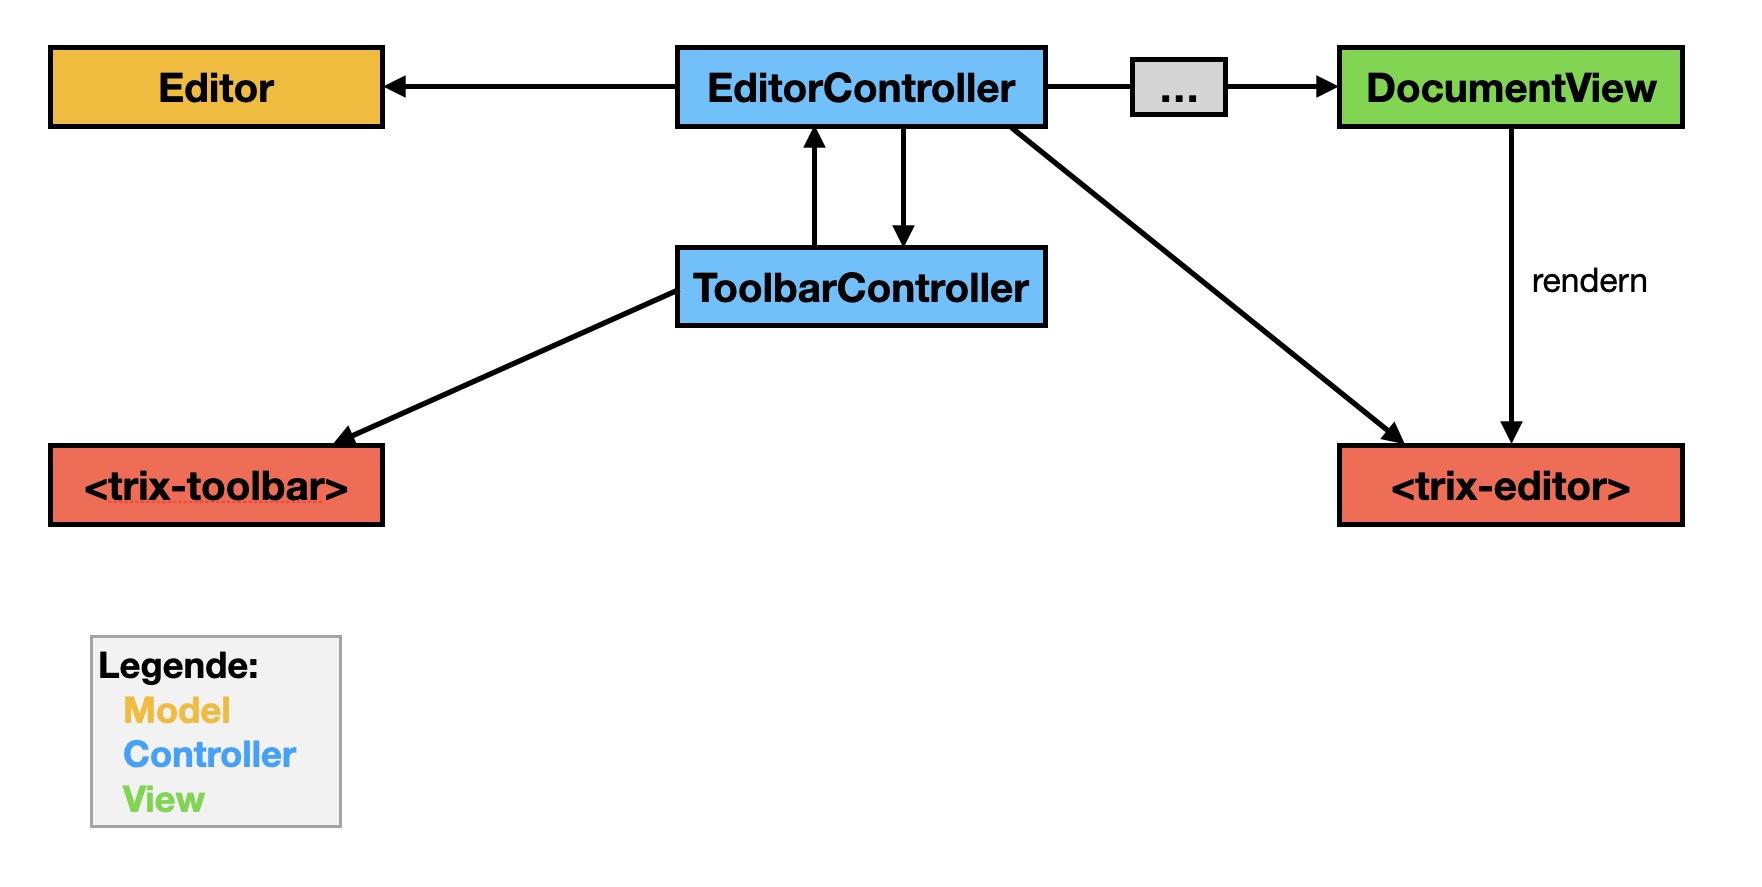
\includegraphics[scale=.4]{images/sysarch.png}
\end{center}
	\caption{Vereinfachte Darstellung der Kommunikation zwischen den Klassen}
\end{figure}

Zur besseren Verständlichkeit wurden nur die Klassen dargestellt, die oberflächlich erkennbar sind. Die Funktionalitäten von Trix unterscheiden sich in ihrer Komplexität von denen der Konkurrenz, da das Dokument auf eine eigene Art und Weise abgespeichert und dargestellt wird. Bei den meisten anderen WYSIWYG Texteditoren wird das Dokument als HTML und bei Trix als ein eigendefiniertes Dokument gespeichert und zur Darstellung in HTML umgewandelt. Außerdem verwendet er den Standard der Web Components (siehe Kapitel \ref{web_comp}). Sobald die Trix Library eingebunden ist, werden ihre benutzerdefinierten HTML-Elemente (\texttt{<trix-editor>}, \texttt{<trix-toolbar>}) registriert. Beim Verwenden eines Trix Editors werden dementsprechend der Controller und in diesem alle weiteren wichtigen Klassen instanziiert, die nicht unbedingt in der Darstellung ersichtlich sind. 

\paragraph{EditorController}\mbox{}\\
Dieser Controller ist eine der Klassen, die umfangreichere Funktionalitäten beinhalten. Er kümmert sich um 

\begin{itemize}
	\item \texttt{InputEvents} bei jeder Tastatureingabe im Editor. Hier wird beispielsweise darauf geachtet, dass beim Einfügen eines Textes dessen Formatierung weiterhin bestehen bleibt.
	\item Formatierungen bei Bedarf und das Aktivieren und Deaktivieren dieser, was aufgrund der Kommunikation zwischen den Controllern auch über die Toolbar möglich ist.
	\item das Rendering, wobei er es im \texttt{DocumentView} auslöst.
\end{itemize}

\paragraph{ToolbarController}\mbox{}\\
Wie auch im Absatz davor erwähnt, kümmert sich dieser Controller um das Aktivieren und Deaktivieren von Formatierungen über die Buttons in der Toolbar. Er hat einen eigenen \texttt{EventListener} auf sich selbst (\texttt{<trix-toolbar>}). Die Besonderheit besteht darin, dass beliebig viele Buttons verwendet werden können. Der Grund dafür ist, dass das Event das sogenannte ``Bubbling`` verwendet. Dies kann man sich wortwörtlich wie eine Blase unter Wasser vorstellen. Wenn ein HTML-Element ein Event besitzt, wird dieses Event auch von HTML-Elementen darunter (Child Elements) ausgelöst. Diese Blase steigt in der Struktur auf und löst das Event aus.\\
Die Buttons haben erst dann eine Funktion, wenn ein selbst definiertes HTML-Attribut hinzugefügt wird. Sobald das Event ausgelöst wird, überprüft der Controller, ob das Attribut vorhanden ist. Wenn das der Fall ist, handelt er anhand des Wertes und formatiert (kursiv) oder löst eine Funktion (rückgängig) aus.

\paragraph{DocumentView}\mbox{}\\
Diese View ist für das gesamte Rendering im Editor zuständig. Das beinhaltet alle Textformatierungen und Textpositionierungen, die auch dementsprechend eine eigene View besitzen, wie etwa TextView für Texte oder AttachmentView für Bilder und Dokumente. Bei jedem Aufruf des Rederings wird das alte Dokument durch ein neues ersetzt.

\section{Motivation}
Der bisher integrierte Browser-UI-Control in Fabasoft Softwareprodukten weist einige Nachteile auf. Der sogenannte ``CKEditor`` in der Version 4 verliert seinen Long Term Support (LTS) im Jahr 2023 (vgl. CKSource, \cite{ckeditor_v4_2020}, 06.09.2020). Dieser wird von der Version 5 abgelöst. Da die neue Version 5 eine neue Lizenz mit sich bringt (vgl. CKSource, \cite{ckeditor_v5_2020}, 06.09.2020), ist dieser Texteditor in den Produkten nicht mehr weiterhin verwendbar. Der Grund dafür ist, dass die neue Lizenz unter den Bedingungen der GNU General Public License Version 2 or later (GPLv2) steht und der Sourcecode auf Nachfrage freigegeben werden muss. Dies entspricht nicht der Philosophie der Firma. Darum wird der Editor durch ein alternatives Produkt abgelöst. Durch eine erste Analyse hat sich herausgestellt, dass sich der Texteditor {\em{Trix}} als Ersatz eignet. Allerdings ist dieser nicht barrierefrei.

\subsection{Gleichstellung von Menschen mit Behinderung}
In der Gesellschaft und im Alltag machen Menschen mit Behinderung oftmals mit kleineren oder größeren Benachteiligungen Bekanntschaft. Global haben etwa 15 Prozent der Weltbevölkerung eine Art von Beeinträchtigung, wobei die rund eine Milliarden Kinder und Erwachsenen assistive Technologien, wie beispielsweise Rollstühle oder Hörgeräte, benötigen. International hat jedes Land eine eigene Definition für den Begriff, weshalb die WHO (vgl. World Health Organisation 2011, \cite{who_disability_2011}) diesen nur grob beschreiben kann. Sie geht dabei immer von drei Punkten aus:

\begin{itemize}
    \item \textbf{Impairment (dt. Schädigung)} bezeichnet jede Anomalie oder jeden Verlust der anatomischen, psychischen oder physiologischen Funktionen und Strukturen des menschlichen Körpers.
    \item \textbf{Disability (dt. Beeinträchtigung)} bezeichnet jeden Mangel oder jede Einschränkung der Fähigkeiten infolge einer Beeinträchtigung, wodurch eine von der Gesellschaft als normal oder in diesem Bereich betrachtete Tätigkeit nicht ausgeübt werden kann.
    \item \textbf{Handicap (dt. Behinderung)} bezeichnet den Nachteil einer Person aufgrund einer Schädigung oder Beeinträchtigung. Eine Behinderung steht im Zusammenhang mit einem Problem mit einer Struktur oder eines Organes des Körpers.
\end{itemize}

\mbox{}\\
''In fact we have a moral duty to remove the barriers to participation, and to invest sufficient funding and expertise to unlock the vast potential of people with disabilities. Governments throughout
the world can no longer overlook the hundreds of millions of people with disabilities who are denied
access to health, rehabilitation, support, education and employment, and never get the chance to shine.'' (vgl. Hawking 2011, \cite{hawking_who_disability_2011})

\mbox{}\\Grundsätzlich wird eine Behinderung in Österreich als dauerhafte Auswirkung einer körperlichen, geistigen oder psychischen Beeinträchtigung oder Beeinträchtigung der Sinnesfunktionen bezeichnet. Diese überschreitet einen Zeitraum von sechs Monaten und erschwert die Teilhabe in der Gesellschaft. Damit die Benachteiligung von Behinderten möglichst flächendeckend beseitigt wird, können diesbezügliche Gesetze auf der Webseite des Rechtsinformationssystems des Bundes (RIS) abgerufen werden:

\begin{itemize}
    \item Das Bundesgesetz über die Gleichstellung von Menschen mit Behinderungen, auch als das Bundes-Behindertengleichstellungsgesetz (BGStG) bezeichnet, zur Regelung der Diskriminierung im täglichen Leben (vgl. RIS, \cite{ris_bgstg_2020}, 30.08.2020).
    \item Das Behinderteneinstellungsgesetz (BEinstG) zur Regelung der Diskriminierung in der Arbeitswelt (vgl. RIS, \cite{ris_beinstg_2020}, 30.08.2020).
    \item Das Bundesgesetz vom 17. Mai 1990 über die Beratung, Betreuung und besondere Hilfe für behinderte Menschen, bekannt als das Bundesbehindertengesetz (BBG) zur Regelung der Aufgaben und Befugnisse des Behindertenanwalts (vgl. RIS, \cite{ris_bbg_2020}, 30.08.2020).
\end{itemize}

\mbox{}\\
Die Fassung des BGStG besagt, dass das Ziel die Beseitigung der Diskriminierung von Menschen mit Behinderungen sei, um diese gleichberechtigt am Leben in der Gesellschaft teilhaben zu lassen und eine selbstbestimmte Lebensführung zu gewährleisten. Der Diskriminierungsschutz gilt somit für diejenigen, die körperlich, geistig, psychisch behindert oder sinnesbehindert sind, ebenso für ihre Angehörigen. Es ist nicht erlaubt jemanden unmittelbar oder mittelbar zu diskriminieren.

\paragraph{Definition: Diskriminierung}\mbox{}\\
Wird eine Person aufgrund ihrer Behinderung in bestimmten Situationen oder gegenüber anderen anders behandelt, so liegt eine unmittelbare Diskriminierung vor. Eine mittelbare Diskriminierung hingegen liegt genau dann vor, wenn neutrale Vorschriften, Kriterien, Verfahren oder Merkmale gestalteter Lebensbereiche den Anschein erwecken, Menschen mit Behinderungen gegenüber anderen auf jegliche Art und Weise zu benachteiligen.\\
Zu diesen Benachteiligungen gehören: 
\begin{itemize}
    \item Barrieren
    \item eine weniger günstige Behandlung
    \item Diskriminierungsaufforderungen
    \item und Belästigung aufgrund einer Behinderung
\end{itemize}

\paragraph{Arten von Behinderungen}\mbox{}\\
Grundsätzlich lassen sich Behinderungen in sechs Kategorien einteilen:

\begin{itemize}
    \item \textbf{Körperliche Behinderungen} kommen am häufigsten vor und nehmen nicht selten mit dem Alter zu. Bezeichnet werden damit starke physische Einschränkungen, die auf eine Dysfunktion oder Schädigung der Stütz- und Bewegungsorgane zurückgeführt werden.
    \item \textbf{Geistige Behinderungen} sind fortwährende, deutlich über dem Durchschnitt liegende Einschränkungen der kognitiven Fähigkeiten und kommen am zweithäufigsten vor. Zu diesen kognitiven Fähigkeiten zählen die Wahrnehmung, die Aufmerksamkeit, das Denken und das Lernen ebenso wie die Erinnerung, die Motivation und die Konzentration.
    \item \textbf{Sinnesbehinderungen} umfassen alle Seh- sowie Hörbehinderungen wie Fehlsichtigkeit, Blindheit, Schwerhörigkeit, Gehörlosigkeit und Taubblindheit.
    \item \textbf{Sprachbehinderungen} oder anders formuliert Störungen des Redeflusses, des Spracherwerbs, des Sprechens und der Stimme bezeichnet all jene Menschen, die nicht fähig sind ihre Muttersprache im entsprechenden Alter schriftlich oder mündlich zu beherrschen.
    \item \textbf{Psychische Behinderungen} umfassen die Beeinflussung des Denkens, Fühlens und Handelns von Menschen. Das heißt wiederum, dass es Abgrenzungen zwischen Verhalten und Erleben gibt.
\end{itemize}

\section{Barrierefreiheit im Web}
\subsection{Definition: Web-Zugänglichkeit}
Web-Zugänglichkeit, oder auch Web Accessibility, bezeichnet, dass alle Menschen auf dem bestmöglichen Weg einen Zugang zu Information oder Dienstleistung im Internet haben. Ziel ist es, Websites und jegliche mobile Anwendungen für alle Nutzerinnen und Nutzer, vor allem auch diejenigen mit Beeinträchtigungen, besser zugänglich und somit barrierefrei zu gestalten. In der heutigen Gesellschaft ist das Internet mit all seinen verfügbaren Leistungen kaum noch wegzudenken. Zahlreiche Dienstleistungen wie etwa Onlinebanking, elektronische Dienste von Instituten und Institutionen, Onlineshop und viele mehr gehören dazu.\\
Das Web-Zugänglichkeits-Gesetz (WZG) umfasst alle rechtlichen Grundlagen zur Erreichung dieses Ziels (vgl. RIS, \cite{ris_wzg_2020}, 30.08.2020). Insbesondere der Bund und alle mit ihm in Zusammenhang stehende Einrichtungen sind dazu verpflichtet barrierefreie Dienstleistungen bereitzustellen. Hierzu gibt es bestimmte Anforderungen:

\begin{itemize}
    \item Wahrnehmbarkeit
    \item Bedienbarkeit
    \item Verständlichkeit
    \item Robustheit
\end{itemize}

\mbox{}\\Des Weiteren wurde ein zeitlicher Anwendungsbereich festgelegt, in dem alle Websites und mobile Anwendungen des Bundes barrierefrei sein müssen:

\begin{itemize}
    \item Neue Websites nach dem 23. September 2018 ab dem 23. September 2019
    \item Alte Websites vor dem 23. September 2018 ab dem 23. September 2020
    \item Alle mobilen Anwendungen ab dem 23. Juni 2021
\end{itemize}

\mbox{}\\Damit diese Dienstleistungen fortlaufend zugänglich sind, müssen die oben genannten Anforderungen regelmäßig überprüft werden. Grundsätzlich hat jede Nutzerin und jeder Nutzer das Recht dazu, sich über Mängel bei Nichteinhaltung der Barrierefreiheit zu beschweren, die dann, wenn sie berechtigt sind, beseitigt werden müssen. 

\section{Aufgabenstellung}
Im Rahmen dieser Diplomarbeit wurde eine Erweiterung für den Texteditor {\em{Trix}} geschrieben, sodass dieser den Ansprüchen für die Produkte der Fa. Fabasoft gerecht wird.  Insbesondere wurden die Kriterien des WCAG 2.1 (Web Content Accessibility Guidelines, siehe Kapitel \ref{wcag_2_1}) erfüllt sowie eine Bedienung mit Screenreadern und vollständig mit Tastatur ermöglicht worden.

\section{Zielsetzung}
Ziel dieser Arbeit war es, den Mitarbeiten und Kunden von der Fa. Fabasoft die Verwendung des Systems weiterhin zu ermöglichen. Der Texteditor sollte weitestgehend von allen Personen einfach und ohne Probleme bedient werden können.

\section{Sollzustand}

\subsection{Erweiterte Systemarchitektur}

\begin{figure}[H]
\begin{center}
	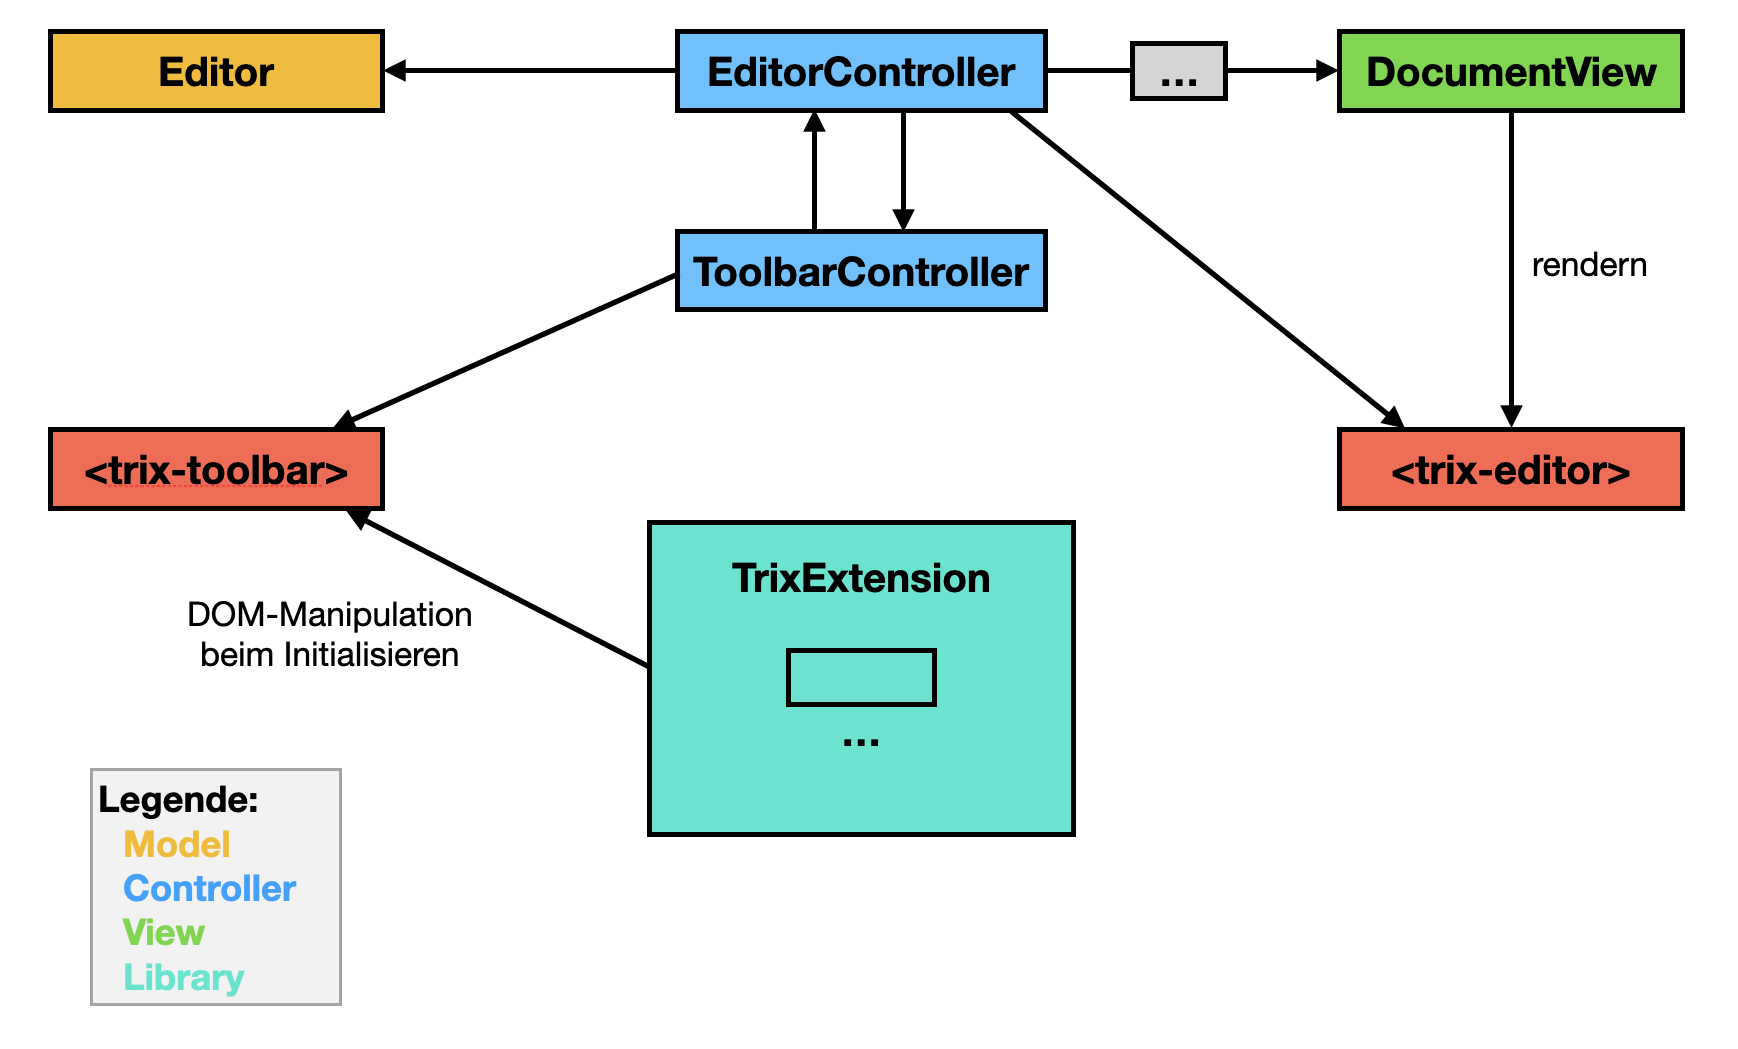
\includegraphics[scale=.4]{images/sysarch_extension.png}
\end{center}
	\caption{Vereinfachte Darstellung der Kommunikation zwischen den Klassen mit der Erweiterung}
\end{figure}

Mit der Erweiterung ``Trix Extension`` ist es möglich, die Toolbar in wenigen Codezeilen robust und sicher zu ersetzen. Hierbei wird der gesamte Inhalt von dem \texttt{<trix-toolbar>} überschrieben. Die Toolbar bestand zuvor aus HTML-Elementen, die statisch in einer JavaScript-Datei definiert waren. Die Struktur der neu ersetzten Toolbar bleibt dennoch dieselbe für Backwards Compatibility. Zusätzlich zu der neuen Anordnungs- und Designmöglichkeit der Buttons werden ARIA-Rollen (Accessible Rich Internet Applications, auch WAI-ARIA) zugeordnet. Des Weiteren werden \texttt{KeyEvents} an \texttt{<trix-editor>} und \texttt{<trix-toolbar>} gehängt. Das Event für den Editor ist sehr simpel, denn er hört auf nur eine Tastenkombination, die es ermöglicht den Fokus auf die Toolbar zu legen. Bei der Toolbar reagiert das Event nur bei Tasten, wie

\begin{itemize}
	\item Pfeiltasten zum Navigieren zwischen den Buttons,
	\item Pfeiltasten mit Steuerung-Taste zum Navigieren zwischen den Button-Gruppen,
	\item Escape-Taste zum Verlassen der Toolbar und zurück Fokussieren des Editors,
	\item Pos1- und Ende-Taste zum Navigieren zum jeweiligen ersten und letzten Button,
	\item und Tab-Taste ignorieren, damit die Nutzer nicht verwirrt werden und die Orientierung verlieren.
\end{itemize}

\subsection{Funktionale Anforderungen}
Für diese Diplomarbeit sind keine funktionalen Anforderungen definiert. Der Grund ist der, dass die Autoren der Meinung sind, dass es keine neuen funktionalen Anforderungen gibt, weshalb die Arbeit schwerwiegend auf nichtfunktionalen Anforderungen basiert.

\subsection{Nichtfunktionale Anforderungen}

\begin{itemize}
	\item Aufsetzen eines npm-basierten Build-Prozesses mit allen notwendigen Artefakten in das Fabasoft npm-Repository.
	\item Aufbau einer Unit-Test-Infrastruktur mit einer Line-Coverage von mindestens 70 Prozent.
	\item Einpflegen der entsprechenden Änderungen zur Erfüllung der Kriterien des WCAG 2.1.
	\item Vollständige Bedienung über eine Tastatur und einen Screenreader.
	\item Einpflegen eines High-Level-APIs, um die Instanzierung und Parametrierung aus dem Fabasoft UI möglichst simpel zu gestalten.
\end{itemize}

\section{Projektablauf und Produkt}
\subsection{Projektablauf}
Im ersten Schritt ist das GitHub Repository des Texteditors Trix geforkt worden, um die notwendigen Änderungen zur Erreichung der Barrierefreiheit einzupflegen. Allerdings sind die Entwickler, die auch die gleichzeitigen Betreuer des Editors sind, bezüglich der Issues und der Pull Requests, sehr inaktiv. Daraufhin wurde mit dem Team der Fabasoft Cloud entschieden, dass eine Erweiterung für den Texteditor sinnvoller ist.

\mbox{}\\Im nächsten Schritt wurde der korrekte Export der bestehenden formatierten Textinhalte in der Fabasoft Cloud ermöglicht. Damit keine zusätzlichen Zeilenumbrüche hinzugefügt und gewisse HTML-Elemente unterstützt und nicht übersprungen werden, sind eine Reihe von Funktionalitäten in Trix selbst und mithilfe von JavaScript Prototypes überschrieben worden. Bei Bedarf können diese Überschreibungen ignoriert werden.

\mbox{}\\Während der Entwicklungsphase dieser Diplomarbeit redigierte ein blinder Mitarbeiter regelmäßig die Funktionen des Texteditors. Zusätzlich zu den Verbesserungsvorschlägen teilte er in seinen Feedbacks mit, welche Kriterien des WCAG 2.1 gut umgesetzt wurden und welche noch erforderlich waren.

\subsection{Produkt}
Mithilfe der Erweiterung ist es möglich, den Texteditor über die Tastatur zu bedienen und somit visuelle Elemente, wie etwa Buttons zum Formatieren des Textes, zu erreichen. 